% Artículo del proyecto: Módem acústico FSK con salto de frecuencia
% Compilar con: pdflatex articulo_modem_acustico.tex (dos veces)
% ANTES DE ENTREGAR: completar los nombres en \Integrantes y la tabla de la prueba física (marcas en rojo).
\documentclass[10pt,twocolumn,letterpaper]{article}
\usepackage[T1]{fontenc}
\usepackage[utf8]{inputenc}
\usepackage{babel}
\babelprovide[import,main]{spanish}
\setlocalecaption{spanish}{table}{Tabla}
\setlocalecaption{spanish}{listtable}{Índice de tablas}
\usepackage{lmodern,microtype}
\usepackage[margin=2cm,columnsep=0.75cm]{geometry}
\usepackage{amsmath,amssymb}
\usepackage{graphicx,xcolor,booktabs,tabularx,multirow,array}
\usepackage[font=small,labelfont=bf,labelsep=period]{caption}
\usepackage{enumitem}
\usepackage{siunitx}
\sisetup{output-decimal-marker={.},group-separator={\,},per-mode=symbol}
\DeclareSIUnit\bit{bit}
\usepackage{tikz}
\usetikzlibrary{positioning,arrows.meta,calc,fit,decorations.pathmorphing}
\usepackage{fancyhdr}
\usepackage[hidelinks]{hyperref}
\setlist{nosep,leftmargin=1.2em}

\definecolor{tx}{HTML}{D23E2A}
\definecolor{rx}{HTML}{1D6BD0}
\definecolor{gris}{HTML}{536173}
\newcommand{\pendiente}[1]{\textcolor{red}{[#1]}}
\newcommand{\Integrantes}{%
  Hans David Zúñiga García\\
  \pendiente{Nombre del integrante 2}\\
  \pendiente{Nombre del integrante 3}}

\pagestyle{fancy}\fancyhf{}
\fancyhead[L]{\small\color{gris}Sistemas de Comunicaciones · Proyecto de aplicación de comunicaciones}
\fancyhead[R]{\small\color{gris}\thepage}
\renewcommand{\headrulewidth}{0.3pt}

\begin{document}

% ------------------------------------------------------------------ portada
\begin{titlepage}
\thispagestyle{empty}\pagestyle{empty}\setlength{\parindent}{0pt}
\vspace*{2.2cm}
{\color{gris}\large\scshape Proyecto de aplicación de comunicaciones}\par\vspace{0.6cm}
{\Huge\bfseries Módem acústico FSK\\[0.25em] con salto de frecuencia\par}
\vspace{0.5cm}
{\Large Transferencia de mensajes cortos entre dispositivos cercanos\\ usando bocina, aire y micrófono\par}
\vspace{1.2cm}
\noindent{\color{tx}\rule{\linewidth}{1.2pt}}\par\vspace{1.2cm}
\begin{tabular}{@{}p{4.2cm}l@{}}
\textbf{Asignatura} & Sistemas de Comunicaciones \\[4pt]
\textbf{Carrera} & Ingeniería en Computación \\[4pt]
\textbf{Facultad} & Facultad de Ingeniería \\[4pt]
\textbf{Semestre} & 2027-1 \\[4pt]
\textbf{Integrantes} & \begin{tabular}[t]{@{}l@{}}\Integrantes\end{tabular} \\[4pt]
\textbf{Fecha de entrega} & 22 de noviembre de 2026 \\
\end{tabular}
\vfill

\begin{tikzpicture}
  \foreach \i/\c in {0/rx,1/tx,2/rx,3/tx,4/rx,5/rx,6/rx,7/rx,8/rx,9/tx,10/tx,11/rx,12/rx,13/tx,14/rx,15/tx,16/rx}
    \fill[\c!80] (\i*0.95,0) rectangle ++(0.8,0.18);
\end{tikzpicture}\par
{\small\color{gris}Preámbulo y palabra de sincronía Barker de 13 bits de cada trama del módem.}
\end{titlepage}

% ------------------------------------------------------------------ página 2
\onecolumn
\pagestyle{fancy}
\section*{Objetivo}
\textbf{El alumno implementará una solución de comunicación al problema de transferir mensajes cortos entre dos dispositivos cercanos que no comparten red, cable ni emparejamiento, usando la tecnología de modulación FSK acústica con salto de frecuencia en una aplicación web que emplea la bocina y el micrófono.}

\medskip
Expresado con un verbo del nivel \emph{Crear} de la taxonomía de Bloom:

\noindent\begin{tabularx}{\linewidth}{@{}>{\bfseries}p{2.3cm}X@{}}
\toprule
Verbo & Diseñar e implementar. \\
Qué & Un módem acústico de modulación por desplazamiento de frecuencia (FSK) binaria con salto de frecuencia, sincronía por palabra Barker y detección de errores CRC-16. \\
Cómo & Con una aplicación web en JavaScript (Web Audio API) que genera los tonos, los reproduce por la bocina, los capta con el micrófono, mide la energía de cada tono con el algoritmo de Goertzel y decide cada bit; validada con una segunda implementación en Python en Google Colaboratory. \\
Para qué & Para transferir mensajes de hasta 120 bytes entre dos computadoras o celulares a pocos metros, sin instalar nada y sin hardware adicional. \\
Por qué & Porque no siempre hay red, cobertura o emparejamiento disponibles, y el sonido es un canal que todos los dispositivos ya tienen; además permite aplicar lo visto en el curso: modulación FSK, ruido, probabilidad de error, sincronía y detección de errores. \\
\bottomrule
\end{tabularx}

\section*{Limitación del estudio}
Nos interesa principalmente usar la tecnología para resolver el problema de transferir mensajes cortos entre dispositivos cercanos sin red, y alcanzar un conocimiento básico de las técnicas de modulación (FSK) y de cómo la tecnología puede usarse para resolver el problema.

El sistema es de una sola vía (simplex), de baja velocidad (50 a 200 bit/s), para distancias de una habitación y sin cifrado. No se diseñó un protocolo de confirmación ni de retransmisión.

\section*{Material}
\noindent\begin{tabularx}{\linewidth}{@{}>{\bfseries}p{4.6cm}X@{}}
\toprule
Computadora portátil & Transmisor o receptor; desarrollo y pruebas automáticas. \\
Google Colaboratory & Cuaderno de validación en Python (NumPy, SciPy, Matplotlib, pandas). \\
Teléfono celular & Segundo equipo (transmisor) y grabadora de audio. \\
Navegador Chrome & Ejecuta la aplicación web (HTML, CSS y JavaScript con Web Audio API). \\
Bocina y micrófono integrados & Transductores del enlace acústico; no se usan cables ni módulos externos. \\
Node.js y Playwright & Pruebas automáticas del módem y de la aplicación en un navegador real. \\
Asistente de IA (Claude) & Apoyo en la programación y en la redacción \cite{claude}. \\
\bottomrule
\end{tabularx}

% ------------------------------------------------------------------ artículo
\twocolumn[
\begin{@twocolumnfalse}
\begin{center}
{\LARGE\bfseries Módem acústico FSK con salto de frecuencia para transferir mensajes cortos entre dispositivos cercanos\par}
\vspace{0.4em}
{\normalsize Aplicación de comunicaciones · Sistemas de Comunicaciones · Ingeniería en Computación · Facultad de Ingeniería\par}
\end{center}
\vspace{0.3em}
\noindent\rule{\textwidth}{0.4pt}
\vspace{-0.6em}
\begin{abstract}
\noindent Se diseñó e implementó un módem acústico que envía texto de un dispositivo a otro por medio de sonido audible, usando únicamente la bocina y el micrófono que ya traen las computadoras y los celulares. El transmisor arma tramas con preámbulo, palabra de sincronía Barker de 13 bits, longitud, número de secuencia, datos y CRC-16, y las modula en FSK binaria de fase continua. Para combatir el eco de las habitaciones, cada símbolo usa el siguiente de cuatro pares de tonos (salto de frecuencia entre 1.6 y 4.4~kHz). El receptor mide la energía de cada tono con filtros de Goertzel, se sincroniza por correlación con el patrón conocido, decide cada bit con un detector no coherente y verifica el CRC. La probabilidad de error de bit medida coincide con la teoría $P_b = \tfrac12 e^{-E_b/2N_0}$ (razón entre 0.89 y 1.07 en dos implementaciones independientes), el sistema entrega el 100\,\% de las tramas de 32 bytes a partir de $E_b/N_0 = 14$~dB, y con eco fuerte el salto de frecuencia mantiene el 96\,\% de tramas correctas contra 14\,\% de la FSK convencional. La velocidad útil es de 80 a 94~bit/s.
\par\smallskip\noindent\textbf{Palabras clave:} FSK, módem acústico, detección no coherente, algoritmo de Goertzel, salto de frecuencia, CRC-16, Web Audio API.
\end{abstract}
\vspace{0.4em}
\noindent\rule{\textwidth}{0.4pt}
\vspace{0.8em}
\end{@twocolumnfalse}]

\section{Introducción}
Compartir un dato corto entre dos dispositivos que están en el mismo cuarto (una dirección, una clave de Wi-Fi, un número de folio) suele requerir que ambos estén conectados a internet, que se emparejen por Bluetooth o que uno escanee un código QR con la cámara. Ninguna de esas opciones funciona siempre: puede no haber cobertura, el emparejamiento es lento o confuso para muchas personas y la cámara necesita que las pantallas estén de frente.

Todos los dispositivos tienen, en cambio, una bocina y un micrófono. Los primeros módems telefónicos ya transmitían datos como tonos audibles: la recomendación V.21 usa FSK a 300~bit/s \cite{v21}, y se han propuesto módems acústicos para computación ubicua \cite{lopes}. Este proyecto retoma la idea con lo visto en el curso: modulación FSK, ruido blanco y probabilidad de error \cite{proakis}, \cite{curso}.

\subsection{Problema social}
Personas en lugares sin cobertura, en emergencias o con poca experiencia tecnológica necesitan pasar información corta entre equipos sin depender de infraestructura ni de configuraciones complicadas.

\subsection{Problema técnico}
Diseñar un enlace digital simplex por un canal acústico que (1) tiene ruido de fondo, (2) atenúa la señal con la distancia, (3) produce eco por las reflexiones en paredes, que en el espectro aparece como desvanecimiento selectivo en frecuencia \cite{kuttruff}, (4) usa relojes de muestreo distintos en el transmisor y el receptor, y (5) debe detectar cualquier trama dañada en lugar de mostrar texto equivocado. Todo debe correr en software, en un navegador, sin hardware adicional.

\section{Requisitos}
\subsection{Requisitos funcionales del enlace}
\begin{table}[h]
\centering\small
\caption{Requisitos funcionales clave.}\label{tab:req}
\begin{tabularx}{\columnwidth}{@{}>{\bfseries}p{2.15cm}X@{}}
\toprule
Alcance & 0.5 a 3~m, dentro de una habitación. \\
Tasa de datos & Mensajes de hasta 120 bytes; al menos 50~bit/s útiles. \\
Latencia & No crítica: menos de 5~s para un mensaje de 32 bytes. \\
Topología & Punto a punto, simplex; cualquier receptor que escuche puede decodificar (difusión). \\
Confiabilidad & Al menos 95\,\% de tramas correctas con $E_b/N_0 \geq 14$~dB y ninguna trama errónea aceptada. \\
\bottomrule
\end{tabularx}
\end{table}

\subsection{Requisitos de software}
\begin{itemize}
\item \textbf{Navegador con Web Audio API} \cite{webaudio} para generar y captar audio en tiempo real, y \textbf{Media Capture} \cite{mediacapture} para abrir el micrófono sin cancelación de eco ni supresión de ruido, porque esos filtros eliminan los tonos.
\item \textbf{Servidor estático con HTTPS} (o archivo local) para publicar la página: los navegadores solo permiten el micrófono en contextos seguros.
\item \textbf{Node.js} para correr el mismo código del módem fuera del navegador y generar resultados de referencia, y \textbf{Playwright} para probar la aplicación en un Chromium real con un micrófono virtual.
\item \textbf{Google Colaboratory} con Python para una implementación independiente que valida los resultados.
\end{itemize}

\section{Herramientas y alternativas}
La Tabla~\ref{tab:alt} resume qué otras opciones existen para el mismo problema y por qué no se usaron.

\begin{table*}[t]
\centering\small
\caption{Alternativas para transferir datos cortos entre dispositivos cercanos y para desarrollar el módem.}\label{tab:alt}
\begin{tabularx}{\textwidth}{@{}>{\raggedright\arraybackslash}p{3.6cm}>{\raggedright\arraybackslash}p{2.5cm}X@{}}
\toprule
\textbf{Opción} & \textbf{Tipo} & \textbf{Por qué no se eligió} \\
\midrule
Bluetooth / BLE \cite{bluetooth} & Radio 2.4~GHz & Requiere emparejar los equipos y permisos del sistema; desde una página web el acceso es limitado. Además, usa salto de frecuencia en radio, la misma idea que aplicamos en audio. \\
NFC & Radio 13.56~MHz & Alcance de pocos centímetros y no todas las computadoras tienen lector. \\
Wi-Fi / Wi-Fi Direct & Radio 2.4/5~GHz & Necesita red o configuración previa; es justo lo que se quiere evitar. \\
Código QR & Óptico & Requiere cámara y que las pantallas estén de frente; no sirve para varios receptores a la vez. \\
ggwave \cite{ggwave} & Biblioteca de datos por sonido & Ya resuelve el problema; usarla no permitiría diseñar la modulación, la trama ni el receptor, que es el objetivo del curso. \\
minimodem \cite{minimodem} & Programa FSK para terminal & Solo corre en Linux desde la terminal, no es visual ni funciona en un celular. \\
MATLAB Communications Toolbox & Simulación & Requiere licencia e instalación, y no transmite en tiempo real desde un celular. \\
GNU Radio & Radio definido por software & Curva de aprendizaje alta e instalación en Linux; está pensado para radios, no para una página web. \\
\midrule
\textbf{Elegido: JavaScript + Web Audio API} & Aplicación web & Corre en cualquier computadora o celular con navegador, sin instalar nada; da acceso directo a las muestras de audio y permite mostrar en vivo cada etapa del módem. \\
\textbf{Elegido: Python en Colab} & Validación & Gratuito y en la nube; con NumPy se vectoriza la simulación de millones de bits. \\
\bottomrule
\end{tabularx}
\end{table*}

\section{Arquitectura del sistema}
La Figura~\ref{fig:bloques} muestra el diagrama de bloques. El transmisor y el receptor son la misma página web; solo cambia la pestaña que se usa.

\begin{figure*}[t]
\centering
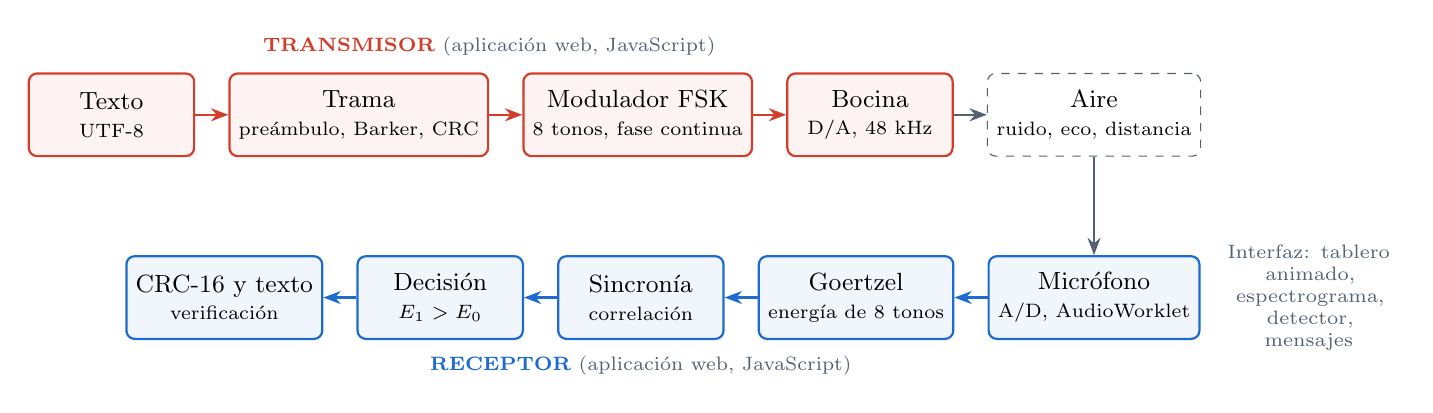
\begin{tikzpicture}[
  blk/.style={draw, rounded corners=3pt, minimum width=2.1cm, minimum height=1.05cm, align=center, font=\small, line width=0.8pt},
  t/.style={blk, draw=tx, fill=tx!6}, r/.style={blk, draw=rx, fill=rx!6},
  ar/.style={-{Stealth[length=2.2mm]}, line width=0.8pt}, lbl/.style={font=\scriptsize\color{gris}, align=center}]
\node[t] (t1) {Texto\\[-1pt]\scriptsize UTF-8};
\node[t, right=0.42cm of t1] (t2) {Trama\\[-1pt]\scriptsize preámbulo, Barker, CRC};
\node[t, right=0.42cm of t2] (t3) {Modulador FSK\\[-1pt]\scriptsize 8 tonos, fase continua};
\node[t, right=0.42cm of t3] (t4) {Bocina\\[-1pt]\scriptsize D/A, 48~kHz};
\node[draw=gris, dashed, rounded corners=3pt, minimum width=2.2cm, minimum height=1.05cm, right=0.42cm of t4, align=center, font=\small] (ch) {Aire\\[-1pt]\scriptsize ruido, eco, distancia};
\node[r, below=1.25cm of ch] (r1) {Micrófono\\[-1pt]\scriptsize A/D, AudioWorklet};
\node[r, left=0.42cm of r1] (r2) {Goertzel\\[-1pt]\scriptsize energía de 8 tonos};
\node[r, left=0.42cm of r2] (r3) {Sincronía\\[-1pt]\scriptsize correlación};
\node[r, left=0.42cm of r3] (r4) {Decisión\\[-1pt]\scriptsize $E_1 > E_0$};
\node[r, left=0.42cm of r4] (r5) {CRC-16 y texto\\[-1pt]\scriptsize verificación};
\draw[ar, tx] (t1) -- (t2); \draw[ar, tx] (t2) -- (t3); \draw[ar, tx] (t3) -- (t4); \draw[ar, gris] (t4) -- (ch);
\draw[ar, gris] (ch) -- (r1); \draw[ar, rx] (r1) -- (r2); \draw[ar, rx] (r2) -- (r3); \draw[ar, rx] (r3) -- (r4); \draw[ar, rx] (r4) -- (r5);
\node[lbl, above=0.08cm of t2.north east, anchor=south] {\textcolor{tx}{\textbf{TRANSMISOR}} (aplicación web, JavaScript)};
\node[lbl, below=0.08cm of r3.south] {\textcolor{rx}{\textbf{RECEPTOR}} (aplicación web, JavaScript)};
\node[lbl, right=0.15cm of r1, anchor=west, text width=2.2cm] {Interfaz: tablero animado, espectrograma, detector, mensajes};
\end{tikzpicture}
\caption{Diagrama de bloques del módem acústico. Todo el procesamiento ocurre en software; el canal es el aire de la habitación.}\label{fig:bloques}
\end{figure*}

\subsection{Trama}
Cada mensaje viaja en una trama (Figura~\ref{fig:trama}) con bits enviados de más a menos significativo:
\begin{itemize}
\item \textbf{Preámbulo} 1010\ldots\ (16 bits): da tiempo a que la bocina arranque y al receptor de medir la señal.
\item \textbf{Sincronía} Barker de 13 bits \cite{barker}: su autocorrelación tiene un pico alto y lóbulos laterales de magnitud 1 como máximo, así que marca el inicio de los datos con precisión.
\item \textbf{Longitud} (8 bits) y \textbf{secuencia} (8 bits): cuántos bytes vienen y qué número de trama es.
\item \textbf{Datos}: de 0 a 120 bytes en UTF-8.
\item \textbf{CRC-16/CCITT} (polinomio $x^{16}+x^{12}+x^5+1$, valor inicial \texttt{0xFFFF}) sobre longitud, secuencia y datos \cite{peterson}.
\end{itemize}

\begin{figure}[h]
\centering
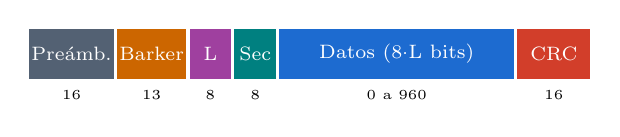
\begin{tikzpicture}[f/.style={draw=white, line width=0.6pt, minimum height=0.65cm, font=\scriptsize, text=white, inner sep=1pt}]
\node[f, fill=gris, minimum width=1.0cm, anchor=west] (a) at (0,0) {Preámb.};
\node[f, fill=orange!80!black, minimum width=0.9cm, right=0pt of a] (b) {Barker};
\node[f, fill=violet!75, minimum width=0.55cm, right=0pt of b] (c) {L};
\node[f, fill=teal, minimum width=0.55cm, right=0pt of c] (d) {Sec};
\node[f, fill=rx, minimum width=3.0cm, right=0pt of d] (e) {Datos (8·L bits)};
\node[f, fill=tx, minimum width=0.95cm, right=0pt of e] (g) {CRC};
\foreach \n/\b in {a/16, b/13, c/8, d/8, g/16} \node[font=\tiny, below=0pt of \n] {\b};
\node[font=\tiny, below=0pt of e] {0 a 960};
\end{tikzpicture}
\caption{Estructura de la trama y número de bits de cada campo. Una trama de 32 bytes dura 3.21~s a 100~bit/s.}\label{fig:trama}
\end{figure}

\subsection{Modulación: FSK con salto de frecuencia}
Cada bit se convierte en un tono de duración $T = 1/R$, con $R \in \{50, 100, 200\}$~bit/s. La fase se acumula de forma continua (CPFSK) para no generar chasquidos. En la variante con salto, el símbolo $k$ usa el par $k \bmod 4$:
\begin{equation}
s(t) = A\sin\!\big(2\pi f_{k \bmod 4,\,b_k}\, t + \phi_k\big),
\end{equation}
con pares $(1600, 2000)$, $(2400, 2800)$, $(3200, 3600)$ y $(4000, 4400)$~Hz. Todas las frecuencias son múltiplos de 50, 100 y 200~Hz, así que los tonos son ortogonales en un intervalo $T$ y no se interfieren entre sí \cite{sklar}. La variante simple usa un solo par, 1800 y 2400~Hz.

La razón del salto es el eco: la cola de un símbolo que rebota en las paredes llega dentro del siguiente intervalo. Con un solo par de tonos, esa cola tiene la misma frecuencia que los datos y confunde al detector; con salto, los tres símbolos siguientes usan otros tonos. Es la misma idea del salto de frecuencia de Bluetooth \cite{bluetooth}, aplicada al audio.

\subsection{Receptor}
\paragraph{Filtros de Goertzel.} Cada $T/8$, el receptor toma una ventana de $N = f_s/R$ muestras y calcula la energía de los 8 tonos con el algoritmo de Goertzel \cite{goertzel}, una DFT de un solo punto:
\begin{gather}
s[n] = x[n] + c\,s[n-1] - s[n-2], \quad c = 2\cos(2\pi f/f_s),\\
E = s_1^2 + s_2^2 - c\, s_1 s_2 = |X(f)|^2 .
\end{gather}
Cuesta $N$ multiplicaciones por tono, contra $N\log_2 N$ de una FFT completa.

\paragraph{Sincronía.} Con $d = (E_1 - E_0)/(E_1 + E_0) \in [-1, 1]$ para el par que corresponde a cada posición, el receptor correlaciona las últimas 21 decisiones (8 bits del preámbulo y el Barker) con el patrón conocido $p_k = \pm 1$:
\begin{equation}
C[m] = \frac{1}{21}\sum_{k=0}^{20} p_k\, d\big[m - 8(20 - k)\big].
\end{equation}
Se declara sincronía cuando $C > 0.65$ y la energía es al menos 5~dB mayor que el ruido promedio medido antes de la trama; se toma el máximo de $C$ en los siguientes $T/2$. Con ruido puro la probabilidad de superar ese umbral en una posición es del orden de $10^{-7}$.

\paragraph{Decisión.} Es un detector no coherente: el bit es 1 si $E_1 > E_0$. En ruido blanco gaussiano su probabilidad de error es \cite{proakis}
\begin{equation}
P_b = \tfrac{1}{2}\, e^{-E_b/2N_0},\label{eq:pb}
\end{equation}
unos 1~dB peor que la FSK coherente, $P_b = Q\big(\sqrt{E_b/N_0}\big)$, pero no requiere conocer la fase de la portadora, que en el aire cambia con cada rebote.

\paragraph{Estimación de $E_b/N_0$.} La energía del par activo incluye la señal y el ruido de dos frecuencias; el ruido promedio por par es el de dos frecuencias, así que $\widehat{E_b/N_0} = 2\,(E_{\text{señal+ruido}}/E_{\text{ruido}} - 1)$. Cada mensaje recibido se muestra con este valor.

\paragraph{Ruido y silencio digital.} El ruido se estima como un promedio exponencial de la energía (constante de 0.5~s) solo mientras no se recibe una trama; los ceros exactos que algunos micrófonos entregan al abrirse no se cuentan como ruido.

\subsection{Interfaz}
La aplicación (Figura~\ref{fig:app}) tiene cuatro pestañas: \emph{Transmitir} (mensaje, ráfaga de prueba y descarga del audio), \emph{Recibir} (micrófono, análisis de una grabación y series de prueba física con exportación a CSV), \emph{Canal simulado} (ruido, eco y diferencia de reloj ajustables) y \emph{Pruebas} (curvas de error contra la teoría). Un tablero animado, al estilo de un circuito, muestra por qué etapa va la señal y explica cada una con su fórmula. La captura del micrófono usa un \emph{AudioWorklet}, que copia las muestras en el hilo de audio y las encola, para no perder bloques cuando la página está ocupada.

\begin{figure*}[t]
\centering
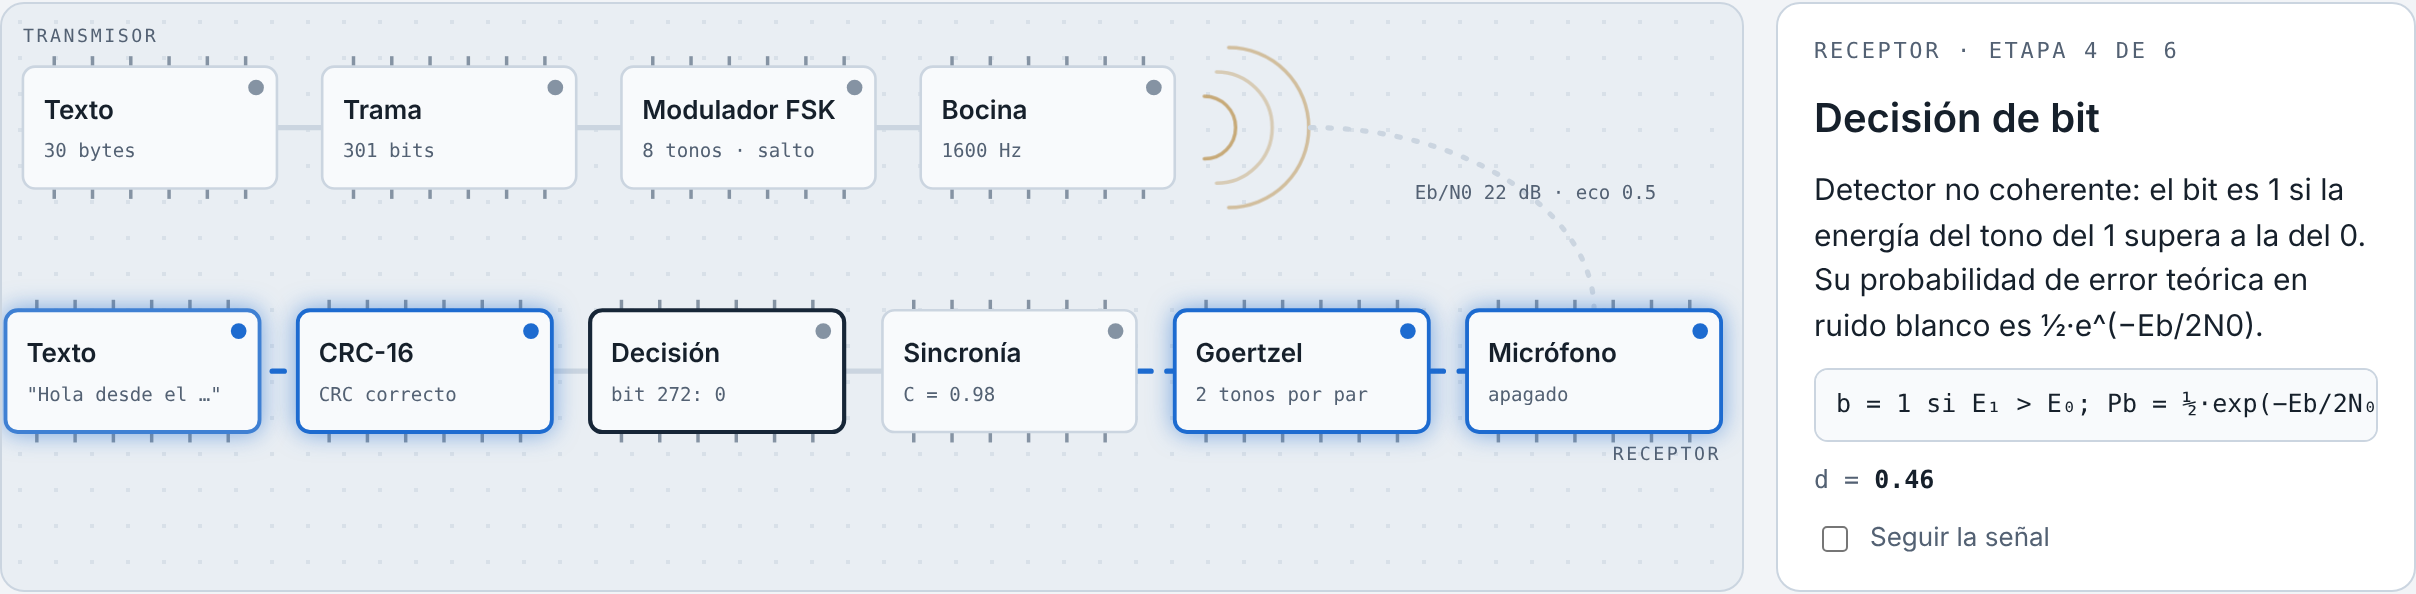
\includegraphics[width=0.92\textwidth]{figs/app_tablero.png}\\[3pt]
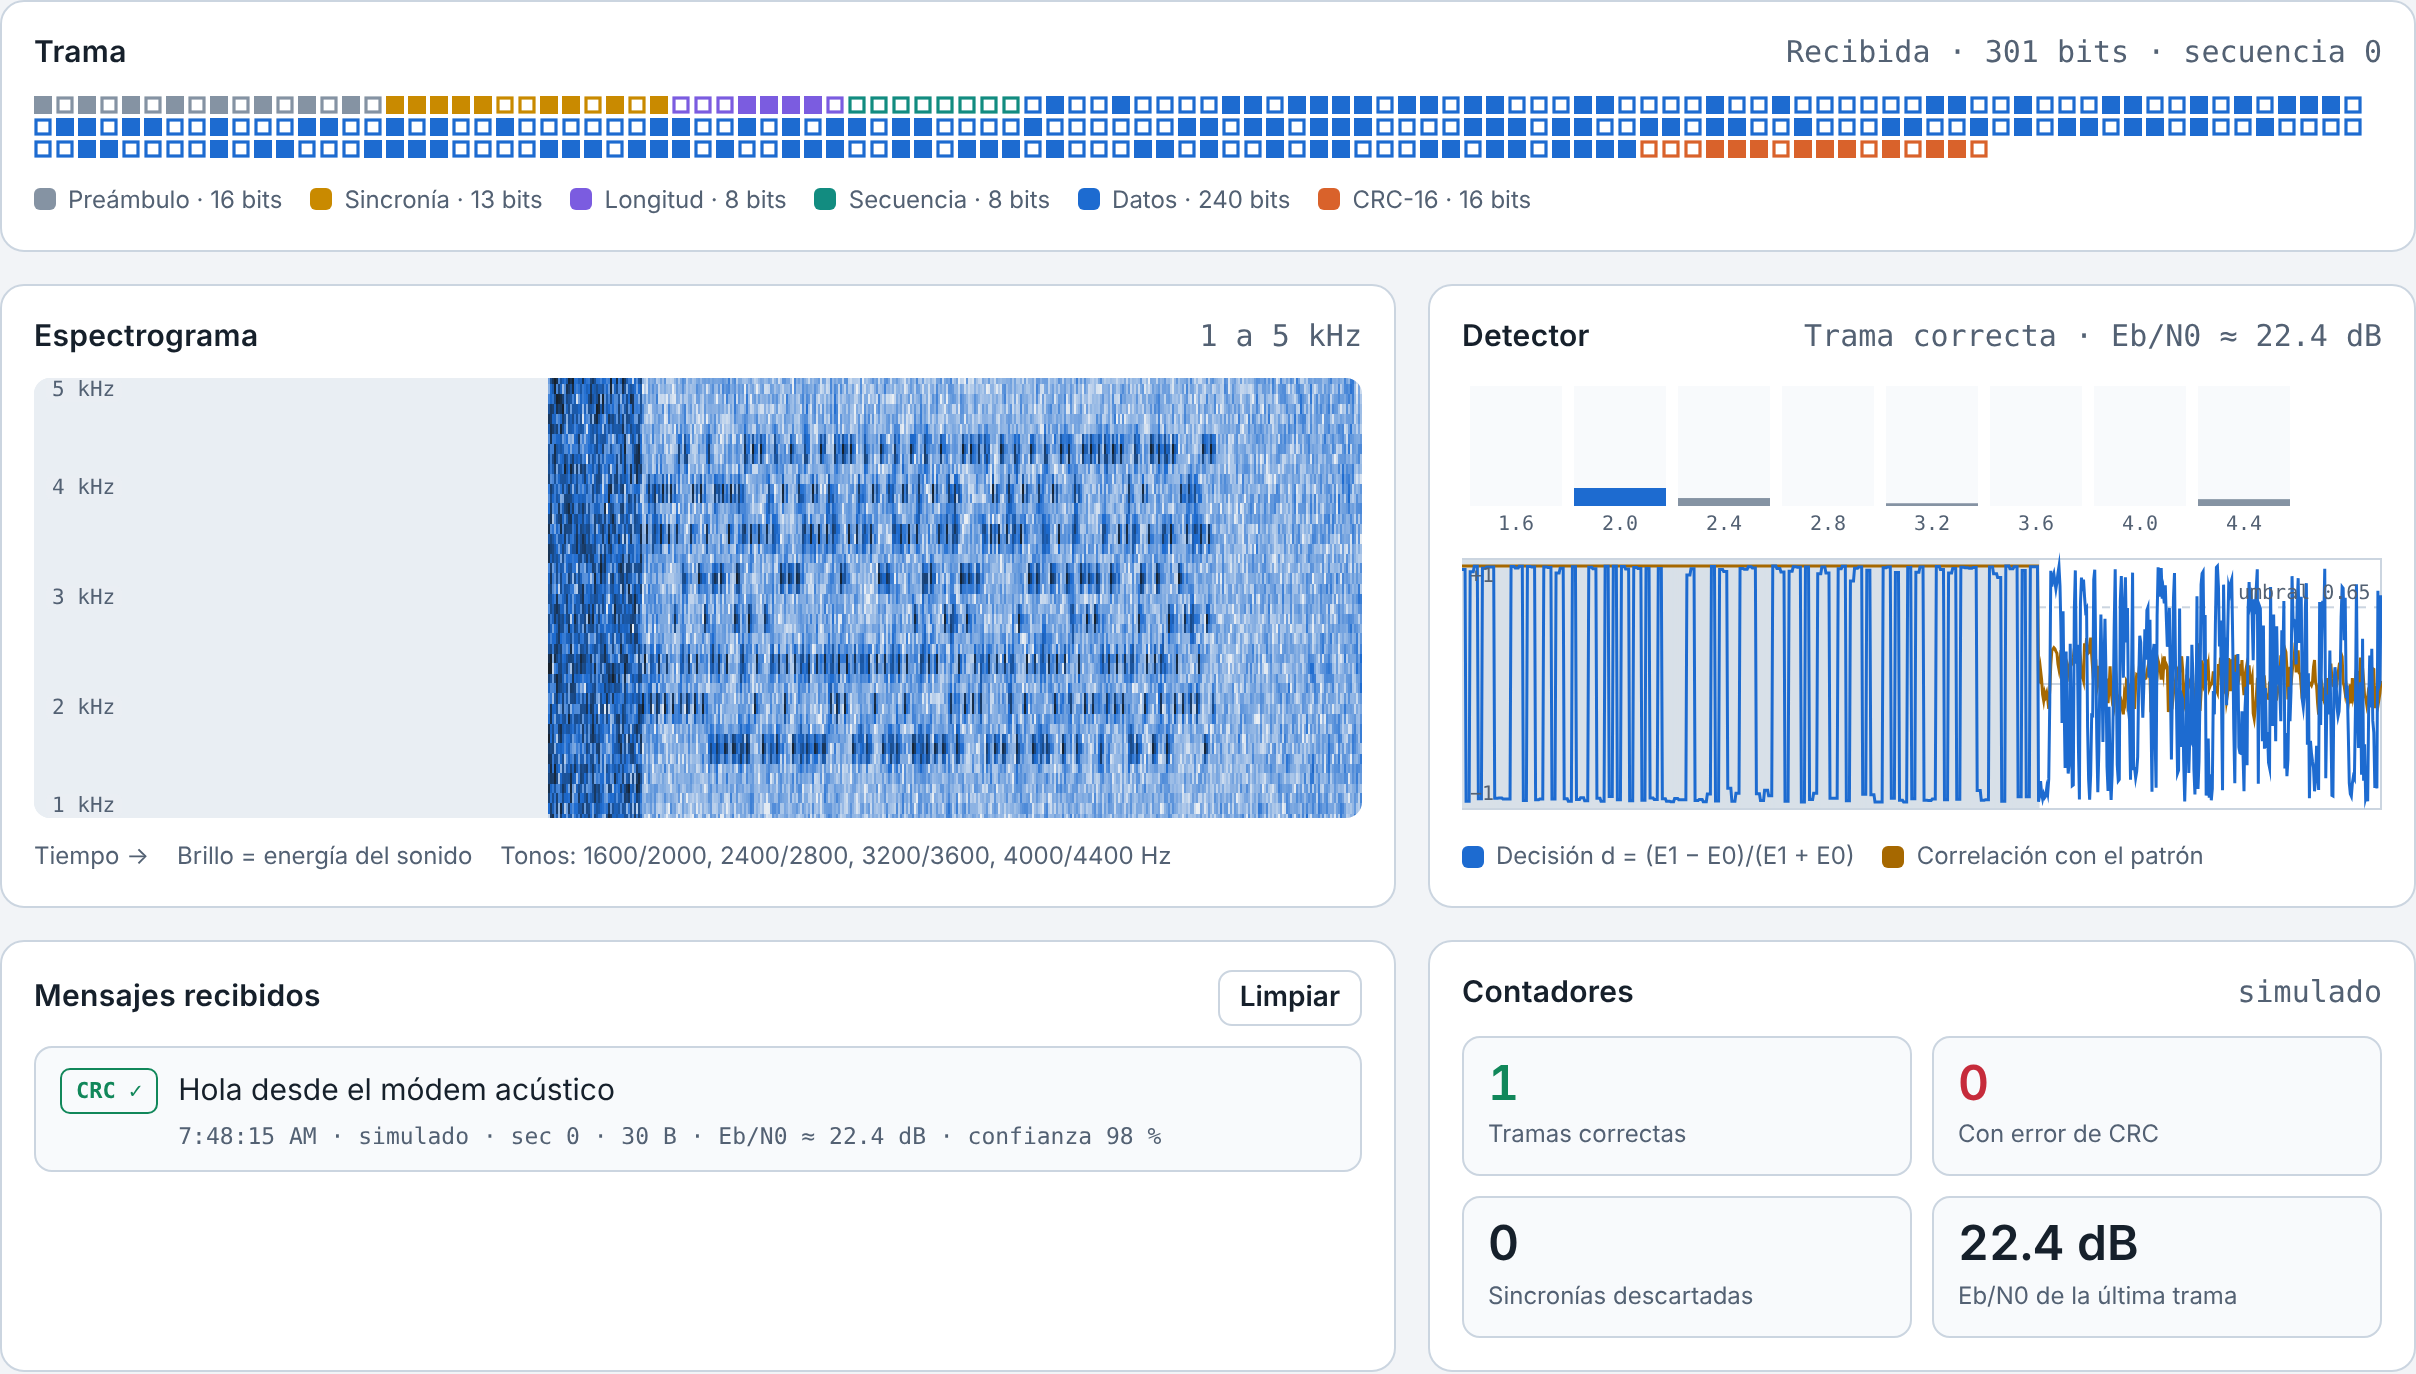
\includegraphics[width=0.92\textwidth]{figs/app_instrumentos_fin.png}
\caption{Aplicación web recibiendo un mensaje por el canal simulado. Arriba, el tablero con el recorrido de la señal (transmisor en rojo, receptor en azul) y la explicación de la etapa activa. Abajo, la trama bit por bit con sus campos, el espectrograma con los ocho tonos, el detector (barras de energía por tono, decisión $d$ y correlación con el umbral) y el mensaje recibido con su CRC y su $E_b/N_0$ estimado.}\label{fig:app}
\end{figure*}

\section{Pruebas de funcionamiento}
Se hicieron pruebas generales del sistema completo, de la entrada de texto a la salida de texto, en tres entornos:
\begin{enumerate}
\item \textbf{Canal simulado} (mismo código JavaScript en Node.js): la señal modulada pasa por ruido blanco con $E_b/N_0$ conocido, eco (14 reflexiones aleatorias entre 2 y 72~ms con decaimiento exponencial) y diferencia de reloj; el receptor en flujo decodifica tramas de 32 bytes con contenido conocido. Se usaron 50 tramas por punto, cada una con una habitación distinta.
\item \textbf{Navegador real con micrófono virtual}: Chromium (Playwright) reproduce como micrófono un archivo con 3 tramas, eco de intensidad 0.6, diferencia de reloj de 80~ppm y $E_b/N_0 = 22$~dB; el navegador lo remuestrea de 48 a 44.1~kHz y la aplicación lo recibe por el AudioWorklet.
\item \textbf{Implementación independiente en Python} (Colab) para la probabilidad de error de bit, el espectro y el eco.
\end{enumerate}
La prueba física con dos dispositivos se describe en la Sección~\ref{sec:fisica}.

\section{Resultados}
\subsection{Pruebas generales}
La Tabla~\ref{tab:func} resume las pruebas generales del sistema completo. Todas pasaron, salvo una trama del micrófono virtual que llegó dañada por el eco y que el CRC marcó como error en lugar de mostrar texto equivocado.

\begin{table}[h]
\centering\small
\caption{Pruebas generales de funcionamiento.}\label{tab:func}
\begin{tabularx}{\columnwidth}{@{}Xr@{}}
\toprule
\textbf{Prueba} & \textbf{Resultado} \\
\midrule
Lazo sin ruido: $f_s$ de 44.1 y 48~kHz, a 50, 100 y 200~bit/s, texto con acentos & 6 de 6 \\
Ráfaga de 5 tramas seguidas & 5 de 5 \\
120~s de solo ruido (falsas tramas) & 0 \\
Diferencia de reloj de 200~ppm & 50 de 50 \\
Micrófono virtual en Chromium (2 vueltas del archivo) & 5 de 6 \\
Audio captado contra tiempo real & 29.00~s en 29.01~s \\
\bottomrule
\end{tabularx}
\end{table}

\subsection{Probabilidad de error contra la teoría}
La Figura~\ref{fig:ber} compara la probabilidad de error de bit del detector con la ecuación~\eqref{eq:pb}. Las dos implementaciones (JavaScript de la aplicación y Python) siguen la curva teórica de 0 a 14~dB; la razón entre la BER simulada y la teórica queda entre 0.89 y 1.07. La misma figura muestra las tramas de 32 bytes con error: el receptor completo, con sincronía incluida, sigue la curva $1 - (1 - P_b)^{288}$, donde 288 son los bits que se demodulan después de la sincronía.

\begin{figure}[t]
\centering
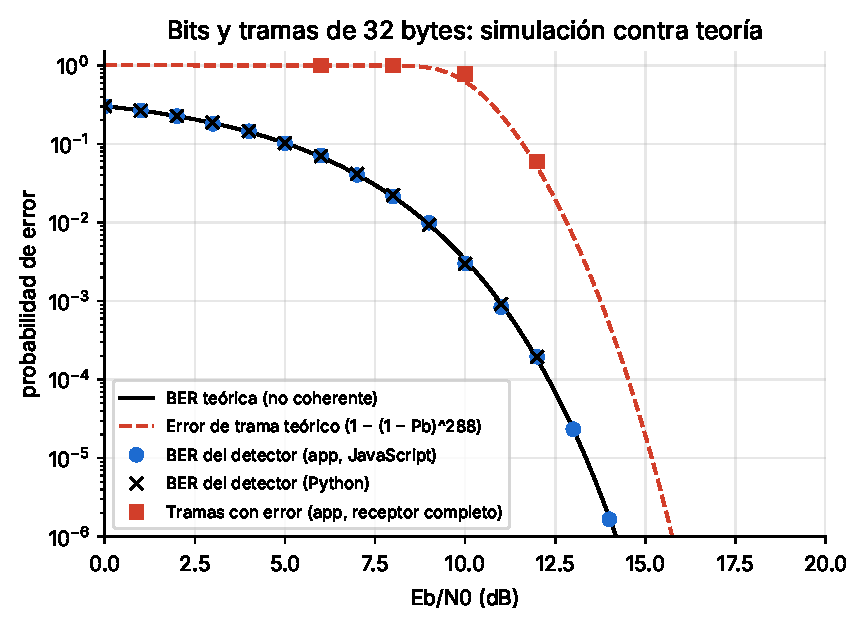
\includegraphics[width=\columnwidth]{figs/ber_per_app.pdf}
\caption{Probabilidad de error de bit y de trama contra $E_b/N_0$. Líneas: teoría; puntos: simulación.}\label{fig:ber}
\end{figure}

\begin{table}[h]
\centering\small
\caption{Tramas de 32 bytes por el canal simulado (50 por punto) y $E_b/N_0$ estimado por el receptor.}\label{tab:per}
\footnotesize\setlength{\tabcolsep}{3.2pt}
\begin{tabular}{@{}rrrrrr@{}}
\toprule
$E_b/N_0$ & Correctas & CRC malo & Perdidas & Teoría & Estimado \\[-1pt]
 & & & & \scriptsize(correctas) & \\
\midrule
6~dB & 0 & 7 & 43 & 0\,\% & 6.2~dB \\
8~dB & 0 & 41 & 9 & 0\,\% & 7.7~dB \\
10~dB & 11 & 37 & 2 & 38\,\% & 9.3~dB \\
12~dB & 47 & 3 & 0 & 95\,\% & 11.5~dB \\
14~dB & 50 & 0 & 0 & 99.9\,\% & 13.6~dB \\
16~dB & 50 & 0 & 0 & 100\,\% & 15.7~dB \\
18~dB & 50 & 0 & 0 & 100\,\% & 17.7~dB \\
20~dB & 50 & 0 & 0 & 100\,\% & 19.7~dB \\
\bottomrule
\end{tabular}
\end{table}

Ninguna trama con bits erróneos se mostró como correcta: todas las que llegaron dañadas las detectó el CRC.

\subsection{Robustez al eco}
La Figura~\ref{fig:eco} es el resultado más importante del diseño. Con eco moderado (0.5) la FSK simple ya pierde el 22\,\% de las tramas; con eco fuerte (1.0) solo entrega el 14\,\%. Con salto de frecuencia se entregan el 98\,\% y el 96\,\%. En Python, con temporización ideal, la BER con eco 1.0 pasa de $1.9\times10^{-1}$ a cero errores en 40\,000 bits.

\begin{figure}[t]
\centering
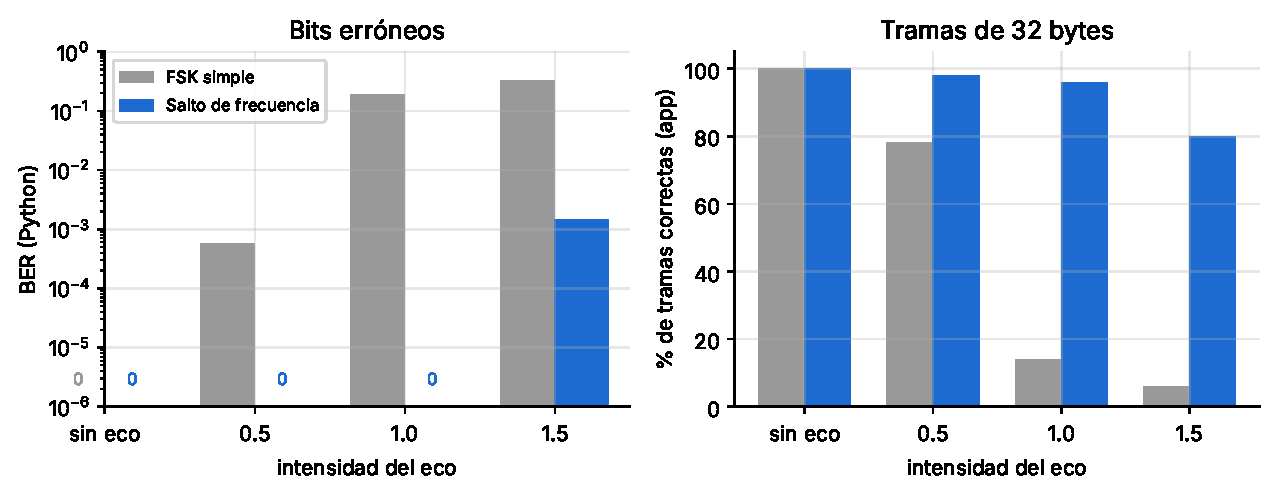
\includegraphics[width=\columnwidth]{figs/eco.pdf}
\caption{Efecto del eco con $E_b/N_0 = 20$~dB. Izquierda: bits erróneos (Python, temporización ideal). Derecha: tramas correctas del receptor completo de la aplicación.}\label{fig:eco}
\end{figure}

\begin{table}[h]
\centering\small
\caption{Tramas correctas (de 50) con salto de frecuencia según la velocidad y el eco, $E_b/N_0 = 20$~dB.}\label{tab:baud}
\begin{tabular}{@{}lrrr@{}}
\toprule
Eco & 50 bit/s & 100 bit/s & 200 bit/s \\
\midrule
0.5 & 50 & 50 & 50 \\
1.0 & 46 & 46 & 42 \\
\bottomrule
\end{tabular}
\end{table}

\subsection{Espectro y ancho de banda}
El salto de frecuencia tiene un costo: el 99\,\% de la potencia ocupa 2988~Hz (de 1.49 a 4.48~kHz) contra 861~Hz de la FSK simple (Figura~\ref{fig:espectro}). El canal acústico de una bocina de celular sobra para ambos. La Figura~\ref{fig:espectrograma} muestra el patrón escalonado de una trama.

\begin{figure}[t]
\centering
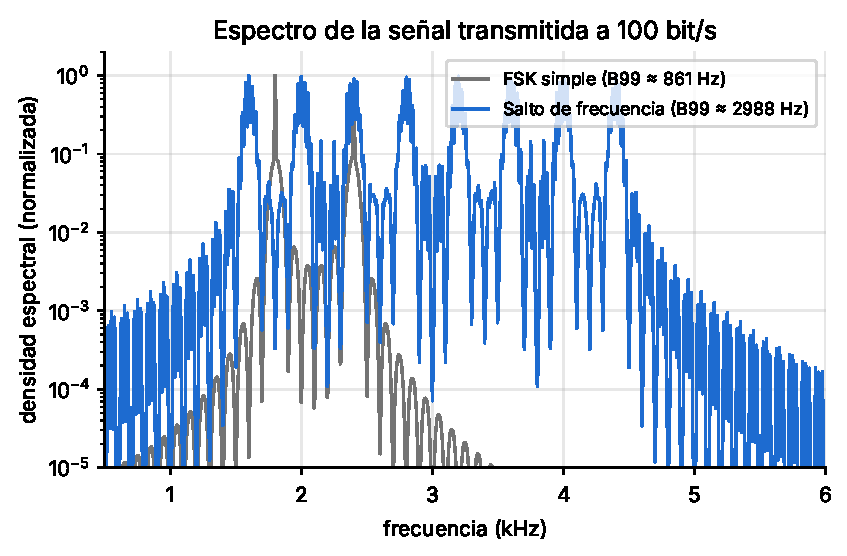
\includegraphics[width=\columnwidth]{figs/espectro.pdf}
\caption{Densidad espectral de potencia a 100~bit/s.}\label{fig:espectro}
\end{figure}

\begin{figure}[t]
\centering
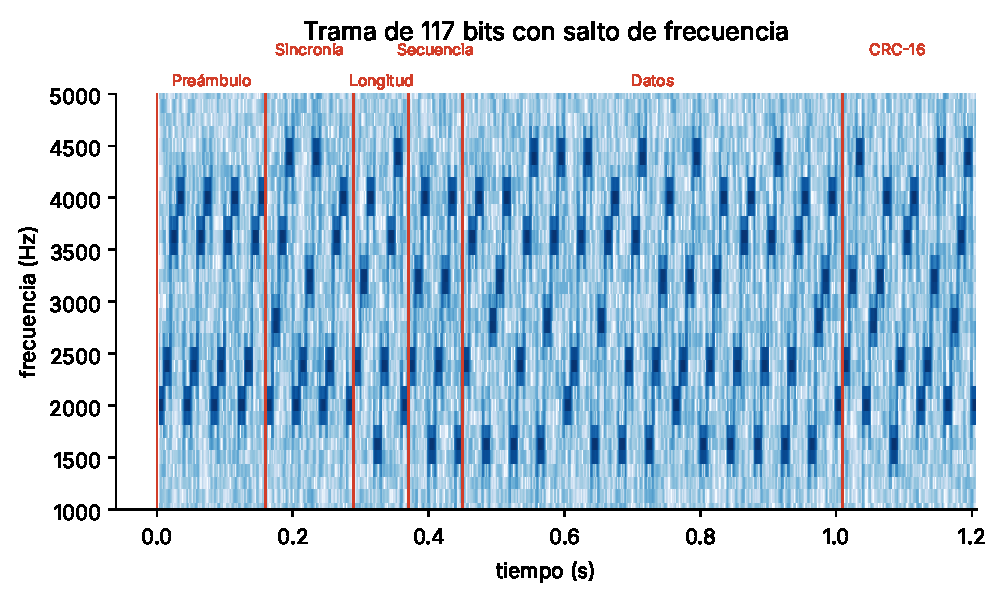
\includegraphics[width=\columnwidth]{figs/espectrograma_trama.pdf}
\caption{Espectrograma de una trama de 117 bits (texto ``Hola FI''): cada símbolo salta al siguiente par de tonos.}\label{fig:espectrograma}
\end{figure}

\subsection{Prueba física con dos dispositivos}\label{sec:fisica}
\textbf{Procedimiento.} El receptor (computadora con Chrome) abre la pestaña \emph{Recibir}, activa el micrófono, anota la distancia y la condición e inicia una serie. El transmisor (celular) envía una ráfaga de 20 tramas de prueba de 32 bytes con contenido conocido, a volumen máximo. La aplicación cuenta las tramas correctas, con error y perdidas, calcula la BER de los datos y el $E_b/N_0$ medio, y exporta un CSV que se analiza en el cuaderno de Colab.

\begin{table}[h]
\centering\small
\caption{Prueba física: 20 tramas de 32 bytes por serie, 100~bit/s, salto de frecuencia. \pendiente{Completar con las mediciones del equipo}}\label{tab:fisica}
\footnotesize\setlength{\tabcolsep}{3.2pt}
\begin{tabular}{@{}llrrrr@{}}
\toprule
Dist. & Condición & Correctas & Perdidas & BER & $E_b/N_0$ \\
\midrule
0.5~m & Silencio & — & — & — & — \\
1~m & Silencio & — & — & — & — \\
2~m & Silencio & — & — & — & — \\
3~m & Silencio & — & — & — & — \\
1~m & Ruido de fondo & — & — & — & — \\
\bottomrule
\end{tabular}
\end{table}

\section{Análisis}
\subsection{Comparación con los requisitos}
\begin{table}[h]
\centering\small
\caption{Resultados contra los requisitos de la Tabla~\ref{tab:req}.}\label{tab:cumple}
\begin{tabularx}{\columnwidth}{@{}>{\raggedright\arraybackslash}p{2.05cm}>{\raggedright\arraybackslash}Xl@{}}
\toprule
\textbf{Requisito} & \textbf{Obtenido} & \textbf{Cumple} \\
\midrule
Alcance & Ver Tabla~\ref{tab:fisica} & \pendiente{—} \\
Tasa de datos & 79.8~bit/s útiles (32~B a 100~bit/s); 93.7 con 120~B & Sí \\
Latencia & 3.21~s de aire para 32~B, más 10~ms de proceso & Sí \\
Confiabilidad & 100\,\% de 14 a 20~dB; 0 tramas falsas & Sí \\
Eco & 98\,\% y 96\,\% con eco 0.5 y 1.0 & Sí \\
Reloj & 200~ppm sin pérdidas & Sí \\
\bottomrule
\end{tabularx}
\end{table}

\subsection{Análisis crítico}
\begin{itemize}
\item \textbf{Tramas a 10~dB.} Se recibieron 22\,\% de tramas correctas contra 38\,\% de la teoría. La teoría supone temporización perfecta; el receptor real busca el inicio en pasos de $T/8$, así que la ventana puede quedar desfasada hasta $T/16$ y pierde algo de energía (unos 0.3~dB). En la zona donde la curva de tramas cae casi vertical, ese corrimiento basta para bajar de 38 a cerca de 22\,\%; además 2 tramas no se sincronizaron. Desde 12~dB la simulación y la teoría coinciden (94\,\% contra 95\,\%).
\item \textbf{Estimación de $E_b/N_0$.} El valor estimado queda entre 0.2~dB arriba y 0.7~dB abajo del real, típicamente 0.3~dB abajo, por la misma pérdida de energía del desfase de la ventana. Es suficiente para comparar las mediciones físicas con la teoría.
\item \textbf{Variación entre habitaciones.} En la aplicación, cada envío al canal simulado usa una sola habitación; algunas tienen reflexiones que cancelan un tono (desvanecimiento selectivo) y fallan varias tramas seguidas. Por eso las estadísticas se hicieron con una habitación distinta por trama.
\item \textbf{Velocidad contra eco.} A 200~bit/s el símbolo dura 5~ms y los 4 pares solo cubren 20~ms de eco; por eso baja a 84\,\% con eco fuerte (Tabla~\ref{tab:baud}).
\item \textbf{Limitaciones de la plataforma.} El micrófono solo funciona con HTTPS o con el archivo local; algunos visores de páginas lo bloquean, por lo que la aplicación permite analizar una grabación del celular.
\end{itemize}

\section{Impacto social}
El módem permite pasar información corta entre equipos que ya tiene la gente, sin red ni accesorios. Beneficia a:
\begin{itemize}
\item \textbf{Comunidades sin cobertura} y \textbf{brigadas en emergencias}, que pueden compartir coordenadas, folios o listas de un equipo a varios a la vez.
\item \textbf{Personas mayores o con poca experiencia tecnológica}, porque no hay que emparejar ni configurar: basta con acercar los equipos.
\item \textbf{Dispositivos de bajo costo} (sensores con un zumbador o un micrófono) que podrían configurarse con sonido en lugar de Wi-Fi o Bluetooth.
\item \textbf{Estudiantes}, porque la aplicación muestra en vivo cada etapa de un sistema de comunicación digital: trama, modulación, espectro, sincronía, decisión y CRC.
\end{itemize}
Es software libre que corre en cualquier navegador, así que el costo para el usuario es cero.

\section{Conclusiones}
Se diseñó e implementó un módem acústico FSK que transmite texto entre dispositivos usando solo la bocina y el micrófono. El detector de Goertzel no coherente alcanza la probabilidad de error teórica de la FSK binaria, el receptor completo entrega todas las tramas de 32 bytes a partir de 14~dB de $E_b/N_0$ y el CRC-16 impide aceptar tramas dañadas. El salto entre cuatro pares de tonos resolvió el principal problema del canal acústico, el eco: con eco fuerte pasó de 14\,\% a 96\,\% de tramas correctas, a cambio de unas tres veces más ancho de banda.

\section{Trabajo a futuro}
\begin{itemize}
\item \textbf{Corrección de errores} (Hamming o Reed--Solomon) para corregir, no solo detectar, los bits dañados.
\item \textbf{Confirmación y retransmisión} (ARQ): que el receptor conteste para volver a pedir tramas perdidas.
\item \textbf{FSK de 4 o más tonos por símbolo} para duplicar la velocidad con el mismo ancho de banda por símbolo.
\item \textbf{Seguimiento de reloj} (detector de Gardner) para tramas más largas, y ecualización del canal.
\item \textbf{Banda casi ultrasónica} (17 a 20~kHz) para que la transmisión no se escuche.
\item \textbf{Cifrado} de los datos y mediciones en más habitaciones y dispositivos.
\end{itemize}

\begin{thebibliography}{99}\small
\setlength{\itemsep}{2pt}
\bibitem[Anthropic; 2026]{claude} ANTHROPIC. \emph{Claude} [Modelo de lenguaje de IA]. Anthropic, 2026. Consultado el 16 de noviembre de 2026. Nota: apoyo en la programación del módem y de las pruebas, y en la redacción de este reporte.
\bibitem[Barker; 1953]{barker} Barker, R. H. (1953). Group synchronizing of binary digital systems. En W. Jackson (Ed.), \emph{Communication Theory} (pp.~273--287). Butterworths.
\bibitem[Bluetooth SIG; 2023]{bluetooth} Bluetooth SIG. (2023). \emph{Bluetooth Core Specification}, versión 5.4.
\bibitem[Cátedra de Sistemas de Comunicaciones; 2026]{curso} Cátedra de Sistemas de Comunicaciones. (2026). \emph{Electronic Communication Systems}, cap.~14 (FSK) y proyecto de computación. Facultad de Ingeniería.
\bibitem[Gerganov; 2020]{ggwave} Gerganov, G. (2020). \emph{ggwave: Tiny data-over-sound library} [Software]. \url{https://github.com/ggerganov/ggwave}
\bibitem[Goertzel; 1958]{goertzel} Goertzel, G. (1958). An algorithm for the evaluation of finite trigonometric series. \emph{The American Mathematical Monthly}, 65(1), 34--35.
\bibitem[ITU-T; 1988]{v21} ITU-T. (1988). \emph{Recomendación V.21: 300 bits per second duplex modem standardized for use in the general switched telephone network}.
\bibitem[Kuttruff; 2016]{kuttruff} Kuttruff, H. (2016). \emph{Room Acoustics} (6.ª ed.). CRC Press.
\bibitem[Lopes y Aguiar; 2003]{lopes} Lopes, C. V., y Aguiar, P. M. Q. (2003). Acoustic modems for ubiquitous computing. \emph{IEEE Pervasive Computing}, 2(3), 62--71.
\bibitem[Mostafa; 2011]{minimodem} Mostafa, K. (2011). \emph{minimodem: general-purpose software audio FSK modem} [Software]. \url{http://www.whence.com/minimodem/}
\bibitem[Peterson y Brown; 1961]{peterson} Peterson, W. W., y Brown, D. T. (1961). Cyclic codes for error detection. \emph{Proceedings of the IRE}, 49(1), 228--235.
\bibitem[Proakis y Salehi; 2008]{proakis} Proakis, J. G., y Salehi, M. (2008). \emph{Digital Communications} (5.ª ed.). McGraw-Hill.
\bibitem[Sklar; 2001]{sklar} Sklar, B. (2001). \emph{Digital Communications: Fundamentals and Applications} (2.ª ed.). Prentice Hall.
\bibitem[W3C; 2021]{webaudio} W3C. (2021). \emph{Web Audio API}. Recomendación del W3C. \url{https://www.w3.org/TR/webaudio/}
\bibitem[W3C; 2024]{mediacapture} W3C. (2024). \emph{Media Capture and Streams}. \url{https://www.w3.org/TR/mediacapture-streams/}
\end{thebibliography}

\end{document}
